\subsection{Comparación de estrategias binarias: BS y BSII}

Para la comparación de los resultados obtenidos con cada una de las estrategias binarias se registran las métricas de precisión, \textit{recall} y \textit{f1-score}. Por claridad se indica que en las gráficas siguientes \ref{fig:Precision} a \ref{fig:F1-score} las etiquetas son:
\begin{itemize}
    \item \textbf{BS\_and:} Búsqueda binaria con conjunción.
    \item \textbf{BS\_or:} Búsqueda binaria con disyunción.
    \item \textbf{BS\_II\_and:} Búsqueda binaria con índice invertido con conjunción.
    \item \textbf{BS\_II\_or:} Búsqueda binaria con índice invertido con disyunción.
\end{itemize}

La precisión (véase figura \ref{fig:Precision}) indica qué porcentaje de los documentos recuperados se consideran relevantes de acuerdo con la etiqueta de la consulta. Como se esperaba los resultados de las estrategias con conjunción (AND) son mejores que los de disyunción (OR). Esto debido a que hay una mayor probabilidad de que si el documento contienen todos los términos de la consulta sea relevante, mientras que si contiene solo uno de ellos, la probabilidad es muchísimo menor.\\ 

\begin{figure}[H]
    \centering
    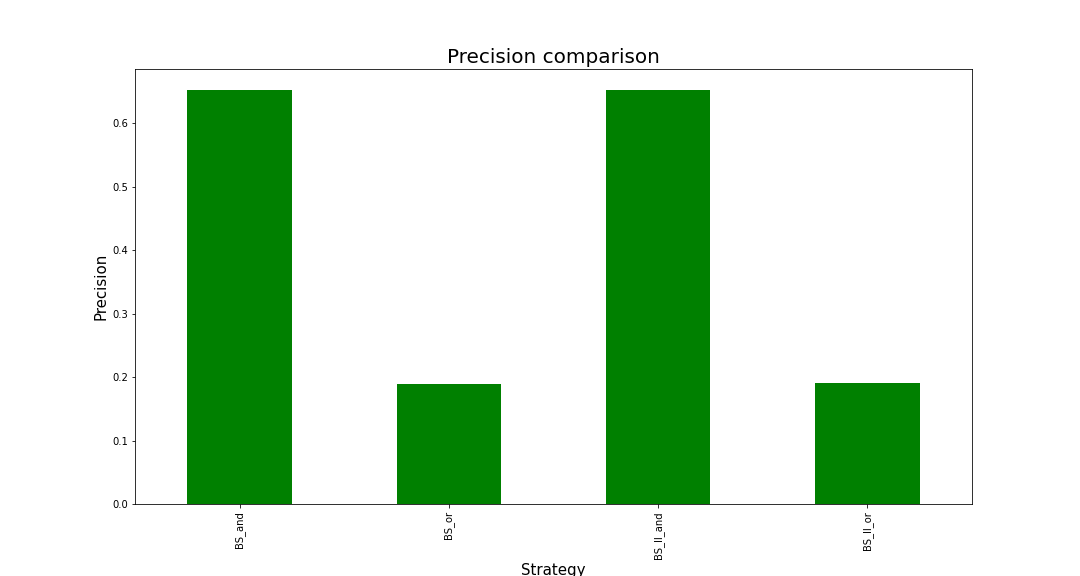
\includegraphics[width=\textwidth]{results/images/BS_precision_comparison.png}
    \caption{Precisión de cada estrategia.}
    \label{fig:Precision}
\end{figure}

El \textit{recall} (véase figura \ref{fig:Recall}), por su parte evalúa qué porcentaje de los documentos relevantes fueron recuperados. Con esto en mente, se espera que el resultado de esta métrica con las estrategias de disyunción sea muy buena, mientras que en las estrategias de conjunción resulta mala. Esto se debe a que existe la posibilidad de que un documento que no contiene todos los términos de la búsqueda sea relevante, por ejemplos sinónimos. Esto ocasiona que la estrategia de conjunción devuelva un valor mucho menor, pues retorna un porcentaje bajo del total de documentos que debería retornar.\\

\begin{figure}[H]
    \centering
    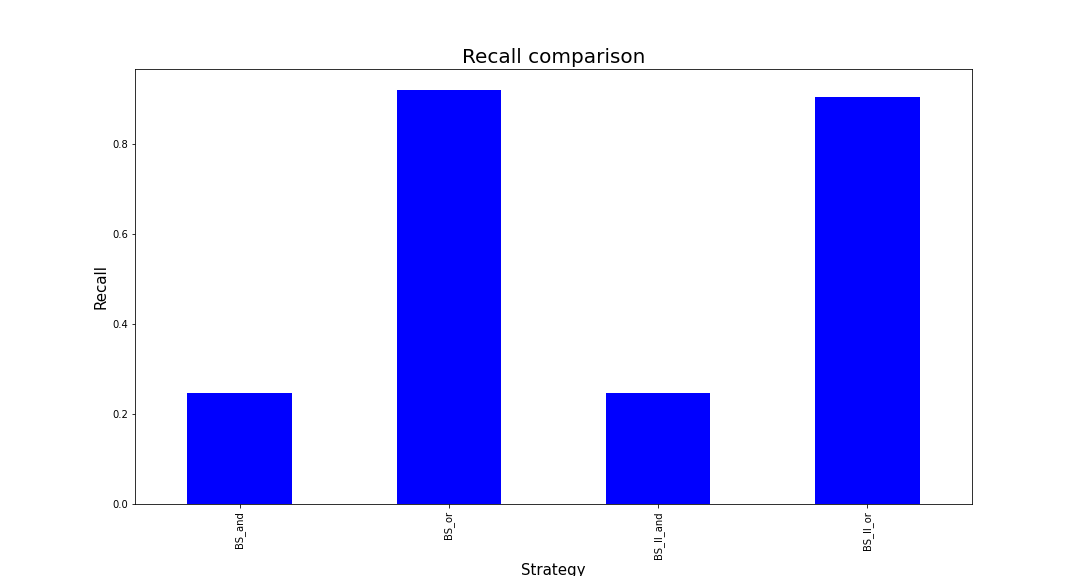
\includegraphics[width=\textwidth]{results/images/BS_recall_comparison.png}
    \caption{\textit{Recall} de cada estrategia.}
    \label{fig:Recall}
\end{figure}

Como se puede observar, las gráficas anteriores evidencian que bajo una de la luz de la métrica de precisión, las estrategias de AND retornan valores muchísimo más altos que los de OR, mientras que para \textit{recall} el resultado de las estrategias disyuntivas son muchísimo mejores. Es por esto que se recurre a una métrica que permita ponderar el resultado de precisión y \textit{recall}. F1-score (véase figura \ref{fig:F1-score}) es una métrica que pondera estos resultados. Se calcula como se muestra en la ecuación \ref{eq:recall}. 

\begin{equation}
    R = \frac{2PR}{P+R}
    \label{eq:recall}
\end{equation}

El resultado es ideal cuando es 1, pues significa que ambas métricas son perfectas. No obstante, es difícil de obtener. El resultado obtenido con las implementaciones actuales indica que el desempeño de las estrategias AND es mejor que el de las OR. Sin embargo, puede resultar conveniente ponderar de manera diferente el peso dado a cada métrica, en caso tal que resulte preferible obtener más documentos relacionados y no únicamente de los que se tenga total certeza de que son relevantes.

\begin{figure}[H]
    \centering
    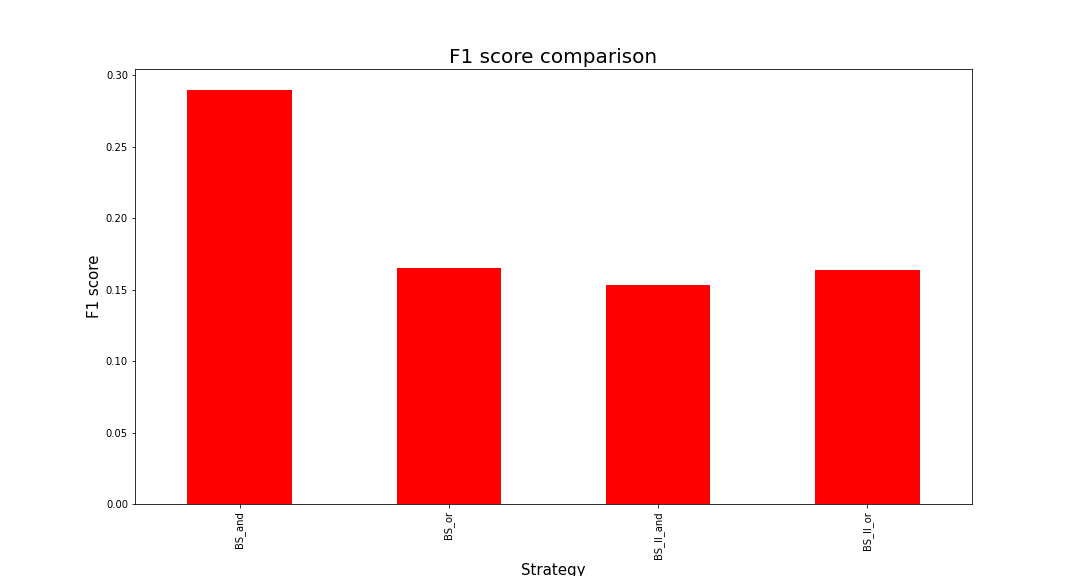
\includegraphics[width=\textwidth]{results/images/BS_f1_comparison.png}
    \caption{F1-score de cada estrategia.}
    \label{fig:F1-score}
\end{figure}

Finalmente, se destaca que los resultados de búsqueda binaria normal y búsqueda binaria con índice invertido son los mismos (para AND y para OR). La única diferencia está en el tiempo de ejecución de cada una, pues el índice invertido da mucha resulta mucho más eficiente. Los tiempos de ejecución para cada estrategia fueron:

\begin{itemize}
    \item \textbf{BS\_OR:} 1.315 s
    \item \textbf{BS\_AND:} 1.289 s
    \item \textbf{BSII\_OR:} 0.00497 s
    \item \textbf{BS\_AND:} 0.00185 s
\end{itemize}

Como es de esperarse, la estrategia de búsqueda binaria con índice invertido es mucho más rápida que la búsqueda binaria con el índice sin invertir. Esto se debe a que en vez de operar con una matriz sobre la cual se debe buscar en qué documento se presenta un término, el índice invertido puede identificar los documentos relevantes directamente a partir del término. 

Teniendo en cuenta las dos estrategias de búsqueda binaria analizadas con sus dos posibles operadores binarios se estableció que hay cuatro términos en los que la búsqueda que requiere el mayor consumo computacional cuando se hacen con la búsqueda binaria. Estas búsquedas corresponden a: \textit{q18}, \textit{q27}, \textit{q40} y \textit{q42}. Las cuatro búsquedas indicadas anteriormente pueden ser consideradas las más caras dado que son las que más términos tienen para la búsqueda. Por otra parte, se considera que la búsqueda binaria es la estrategia con mayor consumo computacional dado que debe recorrer una matriz de tamaño fijo en todas las búsquedas. Sin embargo, no hay una distinción del operador binario que sea utilizado porque la intersección de dos arreglos de tamaño fijo consume los mismos recursos sin importar qué operación binaria se lleve a cabo.

En caso tal que el número de documentos relevantes aumente se presentarían un aumento de costo computacional para las dos estrategias, solo que con condiciones diferentes. Por una parte, la búsqueda binaria debe recorrer todas las posiciones de una matriz por lo que si el tamaño de esta aumenta, el recorrido también lo hará. En este orden de ideas, el consumo computacional para la búsqueda binaria aumentará inevitablemente. Por otra parte, en el caso del índice invertido el aumento del consumo computacional se hará en la medida que los nuevos documentos sean relevantes para los términos. En este caso se podría dar la situación en la que una consulta utiliza términos que no son incluidos en los nuevos documentos, por lo que el consumo computacional para dicha consulta no aumentará. Sin embargo, lo más probable es que los nuevos documentos aumenten la cardinalidad de las listas de posteo, lo cual aumenta a su vez el consumo computacional y el tiempo de respuesta del sistema.

\begin{table}[h]
    \centering
    \begin{tabular}{|c|c|c|c|}
        \textbf{Estrategia} & \textbf{x100} & \textbf{x1000} & \textbf{x10000} \\
        BS\_OR & 131.5 & 1315 & 13150 \\
        BS\_AND & 128.9 & 1289 & 12890 \\
        BSII\_OR & 0.1491 & 0.01988 & 0.02485 \\
        BSII\_AND & 0.00555 & 0.0074 & 0.00925 \\
    \end{tabular}
    \caption{Estimación de tiempos de ejecución para las consultas con un aumento del tamaño de la colección.}
    \label{tab:estimations}
\end{table}

A partir de los tiempos de ejecución presentados previamente, la tabla \ref{tab:estimations} estima nuevos tiempos en función del número de veces en que aumente el tamaño de la colección. Se tiene que un aumento en la búsqueda binaria implicaría que se deben analizar más documentos en la matriz que compone el índice. En este orden de ideas, se espera que haya un aumento lineal del tiempo de ejecución para esta estrategia. En el caso del índice invertido, se tiene que un aumento de la colección no implica un aumento en las listas de posteo. Sin embargo, se espera que estas aumenten de tamaño aunque no de forma lineal. Para modelar un aumento de estas, lo cual va a afectar el tiempo de ejecución, se incluye un aumento en un factor logarítmico. 

Para incluir nuevos documentos en el índice de una búsqueda binaria se deben ejecutar los siguientes pasos:

\begin{enumerate}
    \item Agregar filas al índice con el fin de asociarlos a los nuevos documentos.
    \item Llenar las filas de los nuevos documentos con unos o ceros dependiendo de 
\end{enumerate}



\subsection{Comparación de estrategias clasificadas (\textit{ranked}): RRI, RRDV, GENSIM}

Para evaluar el desempeño de las estrategias de recuperación de la información clasificadas \textit{(ranked)}, se realizó el calculo de las métricas \texttt{P@M}, \texttt{R@M}, \texttt{NDGC@M} y \texttt{MAP} para cada uno de los 35 \textit{queries} en el dataset, donde $M$ representa el número de documentos relevantes en la etiqueta. Para esto se hizo uso de las funciones desarrolladas en la primera parte de este trabajo, las cuales se encuentran en el archivo \texttt{metrics.py}. Como resultado de este proceso se obtuvieron las figuras \ref{fig:rankedP} - \ref{fig:rankedNDCG} y el cuadro \ref{tab:rankedResults} que resume los resultados promedio de todas las estrategias implementadas. \\

En términos generales, se puede observar que los resultados de todas las estrategias \textit{ranked} son bastante buenos. Salvo en dos ocasiones, todas las estrategias son capaces de recuperar al menos un documento relevante para el \textit{dataset} de 35 \textit{queries}. De igual forma, en varios casos se obtienen valores de \textit{precisión}, \textit{recall} y de \textit{NDGC} de 1, lo que representa una recuperación perfecta (se retronaron todos los documentos relevantes en el orden correcto). Vale la pena aclarar que en la mayoría de los casos el resultado de las estrategias de IR, recuperaba muchos más documentos de los que el archivo de etiquetas sugería como relevantes. No obstante, al estar estis resultados ordenados y al hacer la evaluación del desempeño hasta M (salvo por el MAP), se obtiene un desempeño adecuado. 

\begin{figure}[H]
    \centering
    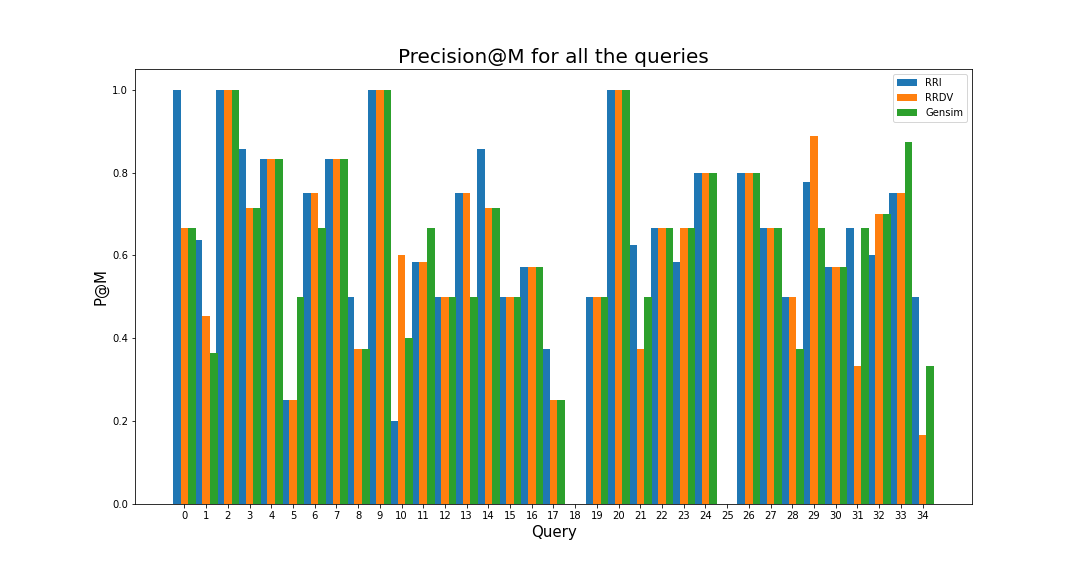
\includegraphics[width=\textwidth]{doc/images/P@M_Ranked.png}
    \caption{Resultados de P@M para todas las \textit{queries} del data set con las estrategias clasificadas (\textit{ranked})}
    \label{fig:rankedP}
\end{figure}

\begin{figure}[H]
    \centering
    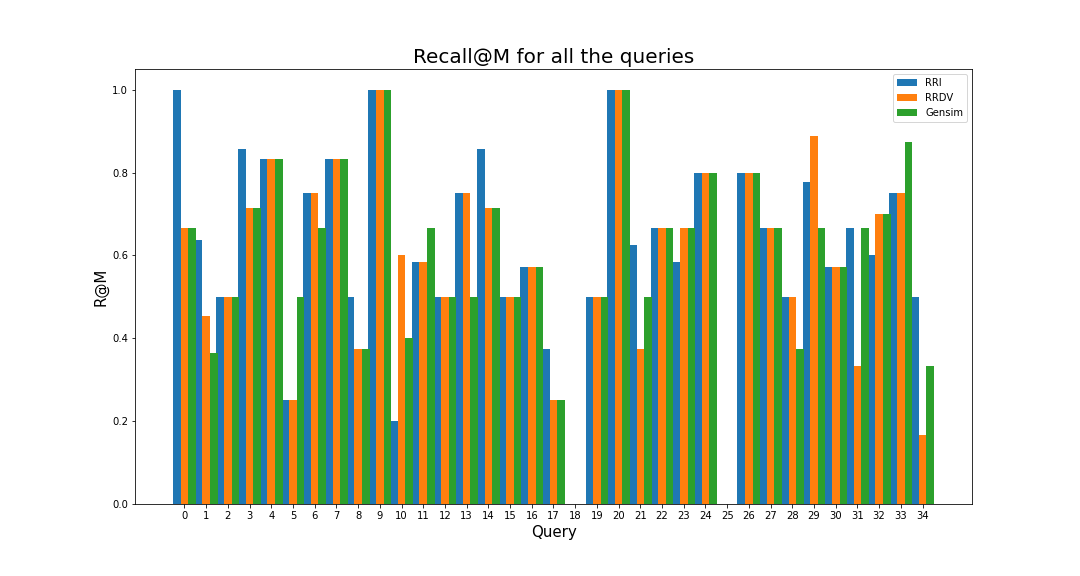
\includegraphics[width=\textwidth]{doc/images/R@M_Ranked.png}
    \caption{Resultados de R@M para todas las \textit{queries} del data set con las estrategias clasificadas (\textit{ranked})}
    \label{fig:rankedR}
\end{figure}


\begin{figure}[H]
    \centering
    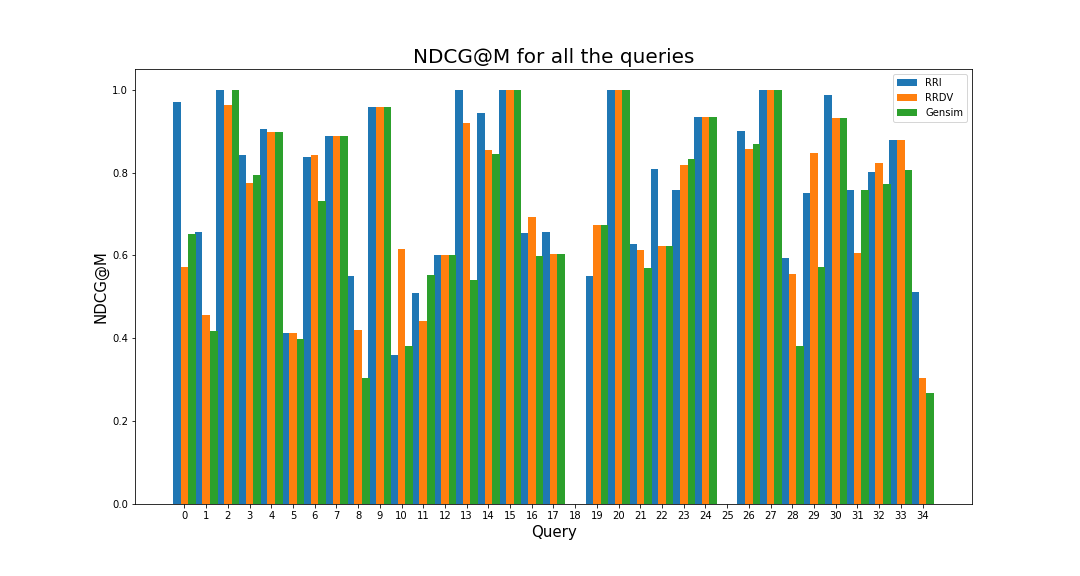
\includegraphics[width=\textwidth]{doc/images/NDCG@M_Ranked.png}
    \caption{Resultados de NDCG@M para todas las \textit{queries} del data set con las estrategias clasificadas (\textit{ranked})}
    \label{fig:rankedNDCG}
\end{figure}

Al momento de comparar el desempeños de las estrategias, se puede observar que, en promedio, RRI presenta mejores resultados que RRDV y Gensim en todas las métricas. Aunque en general los resultados de las 3 estrategias son bastante comparables y sus resultados no difieren en mucho. Adicionalmente, se puede observar que RRDV y Gensim tienen desempeños aun más cercanos, en cuanto a la precisión estos son casi iguales, en cuanto al Recall Gensim es ligeramente mejor y en cuanto al NDCG y al MAP la implementación de RRDV es mejor. \\

Se podría pensar que al aplicar la misma estrategia sobre el mismo \textit{dataset} los resultados deberían ser los mismos. No obstante, existen distintas variaciones que se le pueden aplicar a esta estrategia, la cual cambia sus resultados. Para este caso en especifico, la librería de Gensim, muestra en su documentación distintas formas de pesar las medidas de $tf$, $df$ y realizar la normalización de documentos. Al utilizar la configuración por defecto, se toma como medida de $tf$ el conteo crudo \textit{(raw frequency)} de los términos en el documento, el $idf$ y una normalización de documentos con similaridad coseno. Por su parte la implementación de RRDV realizada es muy similar, pero incorpora un peso logarítmico sobre el $tf$ (véase ecuación \ref{eq:tfidf}). Así las cosas, se podría decir que el efecto de suavizar la frecuencia del $tf$ con la función logaritmo, brinda un beneficio en cuanto al orden de los documentos, pues se obtiene un NDGC@M y un MAP significativamente mayores; pero con una ligera reducción en el desempeño del Recall y una precisión prácticamente igual.

\begin{table}[H]
\centering
\begin{tabular}{|l|c|c|c|c|}
\hline
\textbf{Estrategia} & \multicolumn{1}{l|}{\textbf{Mean P@M}} & \multicolumn{1}{l|}{\textbf{Mean R@M}} & \multicolumn{1}{l|}{\textbf{Mean NDCG@M}} & \multicolumn{1}{l|}{\textbf{MAP}} \\ \hline
\textbf{RRI} & 0.6287 & 0.6144 & 0.7317 & 0.7340 \\ \hline
\textbf{RRDV} & 0.5923 & 0.5780 & 0.6967 & 0.6972 \\ \hline
\textbf{Gensim} & 0.5955 & 0.5812 & 0.6618 & 0.6592 \\ \hline
\end{tabular}
\caption{Resumen de resultados de desempeño para las estrategias clasificadas (\textit{ranked}).}
\label{tab:rankedResults}
\end{table}

Ahora bien, además de su desempeño, las estrategias de RRI y RRDV tienen otras diferencias que vale la pena mencionar. Por un lado, RRDV hace uso del concepto de documentos como vectores, en donde tanto el corpus de documentos, como los \textit{queries} (y en general cualquier agrupación de palabras) son tratados como vectores de un modelo de bolsa de palabras (BOW Model). Por el otro lado, RRI utiliza los pesos de \textit{tf-idf} para comparar puntajes (scores) entre documentos a partir de un \textit{query}. Con esto en mente, el enfoque que propone RRDV puede ser ventajoso por su flexibilidad, pues se puede hacer una comparación de similaridad entre cualquier texto. En este caso, los \textit{queries} y en los documentos se piensan todos en un mismo espacio vectorial, con todas las ventajas que eso conlleva: como la capacidad de crear normas y distancias especificas para la tarea deseada. \\

No obstante, en términos de costo computacional, el enfoque de RRDV parece ser el más costoso. Esto se debe a que típicamente los modelos de bolsa de palabras (BOW) tienen vectores con una alta dimensionalidad (tamaño del vocabulario) y son muy dispersos. Adicionalmente, para realizar la tarea de IR se debe completar un paso adicional de similaridad, el cual conlleva a realizar un producto punto entre dos vectores de este tipo. Al contrastar esto con el enfoque de RRI, en donde solo se debe hacer la suma de los pesos de \textit{tf-idf} (valores ya guardados) sobre los distintos términos del query, los cuales además tienden a ser pocos, da una idea de porque este enfoque puede ser mucho más eficiente. \\

A nivel empírico este racionamiento concuerda con las implementaciones realizadas y se podría probar de forma experimental. Sin embargo, y aunque se cumple de forma evidente en las estrategias implementadas desde cero, el desempeño de Gensim es bastante eficiente. Esto lleva a pensar que existen muchas formas de mejorar la implementación en cuanto a costo computacional y también a que existe un gran número de factores que pueden alterar dicha eficiencia, como el tamaño del vocabulario, el tamaño de los \textit{queries}, el tamaño de los documentos, entre otras cosas. \\

Finalmente, en el caso de que 100 nuevos documentos se incorporen a la colección los cambios requeridos pueden llegar a ser ligeramente distintos a los de una búsqueda binaria. Por un lado, no basta con agregar los documentos bien sea a la matriz de pesos de \textit{tf-idf} o al índice invertido que guarda el tf, sino que es necesario recalcular el $df$, pues ahora se tienen nuevos documentos y la frecuencia con la que las palabras aparecen en los documentos va a cambiar. 


